\chapter{Results}

The results.


\begin{figure}
	\centering
	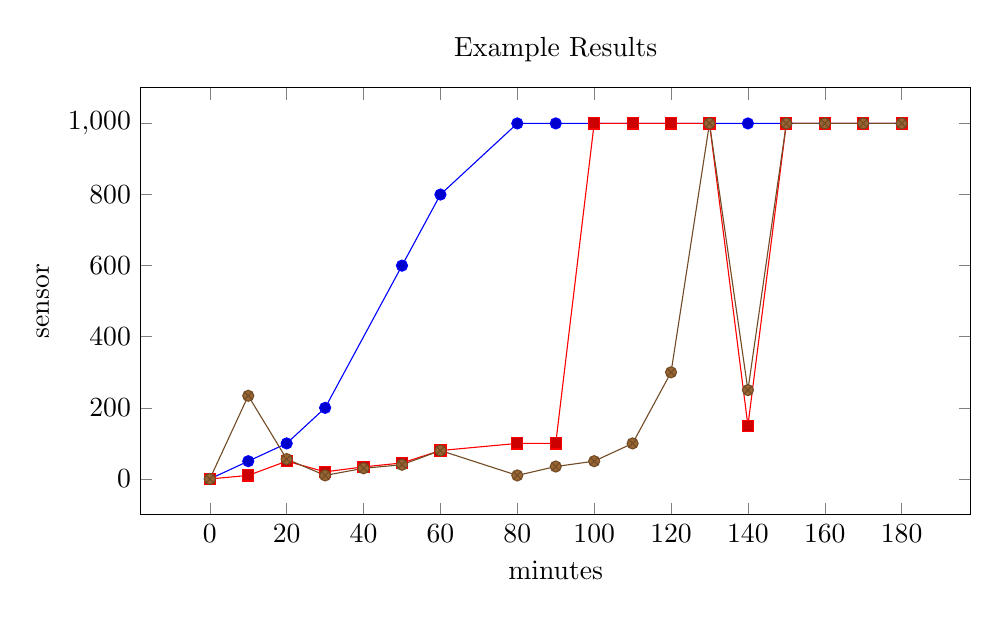
\begin{tikzpicture}
\begin{axis}[
	height=7cm,
	width=\textwidth,
	xlabel=minutes,
	ylabel=sensor,
	title=Example Results,
	unbounded coords=discard],
	
	\addplot coordinates {
		(0,0) 
		(10,50) 
		(20,100) 
		(30,200) 
		(40,inf) 
		(50,600) 
		(60,800) 
		(80,1000)
		(90,1000)
		(100,1000)
		(110,1000)
		(120,1000)
		(130,1000)
		(140,1000)
		(150,1000)
		(160,1000)
		(170,1000)
		(180,1000)
	};
	
\addplot coordinates {
		(0,0) 
		(10,10) 
		(20,50) 
		(30,20) 
		(40,34) 
		(50,45) 
		(60,80) 
		(80,100)
		(90,100)
		(100,1000)
		(110,1000)
		(120,1000)
		(130,1000)
		(140,150)
		(150,1000)
		(160,1000)
		(170,1000)
		(180,1000)
	};	
	
	\addplot coordinates {
		(0,0) 
		(10,234) 
		(20,56) 
		(30,10) 
		(40,30) 
		(50,40) 
		(60,80) 
		(80,10)
		(90,35)
		(100,50)
		(110,100)
		(120,300)
		(130,1000)
		(140,250)
		(150,1000)
		(160,1000)
		(170,1000)
		(180,1000)
	};	
	
\end{axis}
\end{tikzpicture}
 	\vspace{10 mm}
\end{figure}

